\chapter{Operating}
\banner
\chaptquote{Aaron Cohen, NASA administrator}{
	Let's face it, space is a risky business. I always considered
	every launch a barely controlled explosion.
}



\section{Gravity assist}

Consider a spacecraft $\posit{P}$ and a celestial body $\posit{O}$. When
getting close to $\posit{O}$, the gravity will get important enough to
significantly change the trajectory of the spacecraft. The goal is to
get it to turn without using any fuel and while keeping the same velocity
(in a different direction).

\begin{figure}[H]
\centering
\begin{tikzpicture}
\def\ap{0.5}
\node[point=O] (O) at (0,0) {};
\horbit[red,rotate=-45]{O}{\ap}{1.1}{0.5}
\node[point=X] (X) at (-45:-\ap) {};
\end{tikzpicture}
\caption{
	The speed of the mobile will increase as it heads towards the
	periapsis $\posit{X}$, trading its gravitational potential for
	kinetic energy; it will then decrease when moving away from
	$\posit{X}$. Overall, the total energy will be conserved and it
	will move as fast when leaving $\posit{O}$ as when getting there.
}
\end{figure}

Now, this velocity change is done relatively to $\posit{O}$.

\begin{figure}[H]
\centering
\begin{tikzpicture}
\def\ap{0.5}
\def\rad{4}
\orbit[blue]{0,0}{\rad}{\rad}{135}{45}
\node[point=O] (O) at (0,\rad) {};
\horbit[red,rotate=-45]{O}{\ap}{1.1}{0.5};
\draw (-3,4) edge[->] node[pos=1,right]{$x$} +(1,0)
             edge[->] node[pos=1,above]{$y$} +(0,1);
\end{tikzpicture}
\caption{
	If we note $\speed{v_P}$ the velocity of $\posit{P}$ relatively
	to $\posit{O}$ and $\speed{v_O}$ the velocity of $\posit{O}$
	around its primary, the velocity of $\posit{P}$ around
	$\posit{O}$'s primary is $\speed{v_P}$ before encountering
	$\posit{O}$ and $\speed{v_P} + \speed{v_O}$ after (note that
	the \textcolor{red}{red} trajectory moves with $\posit{O}$
	along the blue trajectory).
}
\end{figure}

\begin{figure}[H]
\centering
\begin{subfigure}{\textwidth}
	\centering
	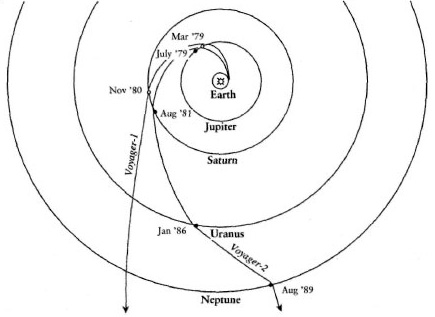
\includegraphics[width=0.8\linewidth]{img/ast-voyager-orbits.jpg}
	\caption{
		Voyager 2 flew by Jupiter, Saturn, Uranus and Neptune,
		but the swingby of Neptune actually slowed down the
		vessel as it turned slightly out of the trajectory
		(out of the plane in the image). \cite{voyagerassists}
	}
\end{subfigure}
\begin{subfigure}{\textwidth}
	\centering
	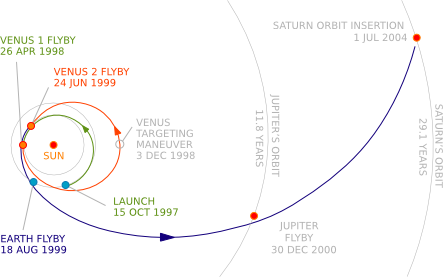
\includegraphics[width=\textwidth]{img/cassiniorbit.png}
	\caption{
		The Cassini-Huygens spacecraft left the Earth for the
		\textcolor{green}{green} solar orbit (\delay{1997});
		it then flew twice by Venus to increase its orbit to
		the \textcolor{red}{red} one (\delay{1998}) and then
		to the \textcolor{blue}{blue} one (\delay{1999}). The
		\textcolor{blue}{blue} trajectory was further improved
		by gravity assists by the Earth (\delay{1999}) and by
		Jupiter (\delay{2000}). \cite{cassiniassists}
	}
\end{subfigure}
\caption{Two famous series of gravity assists}
\end{figure}



\section{Rendez-vous}

The goal of rendez-vous is to make the position \textbf{and velocity}
of a spacecraft $\posit{P1}$ roughly matching those of $\posit{P2}$. Once
the spacecrafts have performed a rendez-vous, they can do useful action
such as docking or crew transfer.

\begin{remark}
After rendez-vous, two vessels would be moving along a very similar
orbit. On short durations (compared to the orbital periods), the pull
of gravity can simply be ignored like if the vessels were subject to no
force at all (making docking simple).
\end{remark}

Same position and same velocity means a similar orbit. Once both
satellites are revolving around the same body, the first correction is
that of inclination: one will perform an inclination change (either
(anti-)normal burn, straight burn, or bi-elliptical). When they are
orbiting in the same plane, they will have to consort their orbits,
and synchronize on the final orbit.

A simple way to do this is to have the orbits joining in one point (say,
the periapsis) while their period is significantly different. After a
few revolutions, the two spacecraft will get in the common point at the
same time and will be able to join their orbit. It is handy to correct
the orbits before the last revolution to get a more accurate rendez-vous.

\begin{figure}[H]
\centering
\begin{tikzpicture}
\def\peri{2}
\def\apoa{3}
\def\apob{5}
\node[point=O] (O) at (0,0) {};
\node[loint=X] (X) at (-\peri,0) {};
\orbit[blue]{O}{\apoa}{\peri}{0}{360};
\orbit[red] {O}{\apob}{\peri}{0}{360};
\orbitpoint[point=P1]{O}{\apoa}{\peri}{ 40}{P1}{};
\orbitpoint[point=P2]{O}{\apob}{\peri}{110}{P1}{};
\end{tikzpicture}
\caption{
	$\posit{P2}$ will reach $\posit{X}$ ahead of $\posit{P1}$;
	however, the red orbit has a higher apoapsis and thus a
	longer period: after some time, $\posit{P1}$ will catch up
	with $\posit{P2}$
}
\end{figure}



\section{Satellite coverage}

Assume we want to set up a satellite network around a body
$\posit{O}$. The coverage is done with satellites in circular orbits. It
is handy to have several satellites around the same orbit; to cover a
band on the surface at all time. The fist thing to ensure is that the
satellites stays connected.


\subsection{Connectivity}

We are interested in two values: the closest approach of the
lines-of-sight to $\posit{O}$, notated $\dist{h}$, that must be greater
than the radius of the body $\dist{R}$ and the distance between the
satellites, notated $\dist{s}$ that must be lower than the range of the
satellites antennas $\dist{r_a}$.

\begin{figure}[H]
\centering
\def\n{5}
\begin{tikzpicture}
\def\R{2}
\def\r{3}
\pgfmathsetmacro{\h}{cos(180/\n)*\r}
\node[point=O] (O) at (0,0) {};
\node[point=C] (C) at (180/\n:\h) {};
\draw[blue] (O) circle (\R);
\orbit[red]{O}{\r}{\r}{0}{360};
\foreach \i in {1,...,\n}
{
	\orbitpoint[point=P\i]{O}{\r}{\r}{(\i-1)*360/\n}{P\i}{}
}
% inspired from http://tex.stackexchange.com/questions/75146/draw-a-path-between-many-nodes-using-foreach/75149#75149
\foreach \i  [remember=\i as \lasti (initially \n)] in {1,...,\n}
{
	\draw[green] (P\lasti) -- (P\i);
}
\draw (O) --node[below]     {$\dist{r}$} (P1);
\draw (O) --node[above left]{$\dist{h}$} (C);
\markangle{P1}{O}{C}{$\alpha/2$}{1}
\draw (P3) -- (O) -- (P4);
\markangle{P3}{O}{P4}{$\alpha$}{1}
\draw[green] (P4) --node[below]{$\dist{s}$} (P5);
\end{tikzpicture}
\caption{
	There are $\n$ satellites on the \textcolor{red}{red} orbit around
	$\posit{O}$. The surface is shown in \textcolor{blue}{blue} and
	the lines-of-sight of the satellites in \textcolor{green}{green}.
}
\end{figure}

What we have to choose is the number of satellites $n$ and their
distance from $\posit{O}$, $\dist{r}$. With, $\angle{\alpha} = \frac
{\angle{2\pi}} n$ and simple trigonometry, we get that:
\[
\dist{h}
= \dist{r} \cos \frac {\angle{\alpha}} 2
= \dist{r} \cos \frac {\pi} n
\]
and
\[
\dist{s}
= 2 \dist{r} \sin \frac {\angle{\alpha}} 2
= 2 \dist{r} \sin \frac {\pi} n
\]

Thus, with the requirement that $\dist{h} > \dist{R}$ and $\dist{s} >
\dist{r_a}$, we need:
\[
\frac {\dist{R}} {\cos \frac {\pi} n}
<
\dist{r}
<
\frac {\dist{r_a}} {2 \sin \frac {\pi} n}
\]

Conversely, if we want to know the the necessary value of $n$ for a
given altitude $\dist{r}$, we have to ensure that:
\[
n
\ge
\frac {\pi} {\arccos \frac {\dist{R}} {\dist{r}}}
\text{ and }
n
\ge
\frac {\pi} {\arcsin \frac {\dist{r_a}} {2 \dist{r}}}
\]

\begin{remark}
Functions $\arccos$ and $\arcsin$ are only defined from $-1$ to $1$
meaning that we need that $\dist{r} > \dist{R}$; this makes sense.
Moreover, when $2 \dist{r} < \dist{r_a}$, the second conditions should
be ignored, since it means the whole orbit stays in range.
\end{remark}

Similar information is available on the KSP wiki \cite{coverage}.


\subsection{Coverage}

The curvature of Kerbin makes that a satellite sees less than half the
surface; the closer it is the surface, the less it can see.

\begin{figure}[H]
\centering
\begin{tikzpicture}
\def\R{2}
\def\r{5}
\node[boint=O] (O) at (0,0) {};
\node[point=P] (P) at (\r,0) {};
% tangents
\pgfmathsetmacro{\be}{acos(\R/\r)}
\node[point=X1] (X1) at ( \be:\R) {};
\node[point=X2] (X2) at (-\be:\R) {};
\draw (P) -- (X1);
\draw (P) -- (X2);
% values
\draw (O) --node[above left]{$\dist{R}$} (X1);
\draw (O) --node[below]     {$\dist{r}$} (P);
\markangle{X1}{P}{O}{$\alpha$}{1}
\markangle{X1}{O}{P}{$\beta$} {1}
% show covered area
\fill[grey!10] (P) -- (-\be:\R) arc (-\be:\be:\R) -- cycle;
\draw      ( \be:\R) arc ( \be:360-\be:\R);
\draw[red] (-\be:\R) arc (-\be:\be    :\R);
\end{tikzpicture}
\caption{
	$\posit{X1}$ and $\posit{X2}$ are the farthest point that
	$\posit{P}$ can see from this distance; the line $(PX1)$ is
	said to be tangent to the circle, and there is a right angle
	in $\posit{X1}$
}
\end{figure}

\begin{remark}
This property is used on the surface: the crow's nest is an observation
spot located high in the masts of a ship to see significantly farther
away. The distance you can see from altitude $\dist{a}$ is $\dist{R}
\arccos \frac {\dist{R}} {\dist{R} + \dist{a}}$.
\end{remark}

We quickly see that $\sin \angle{\alpha} = \cos \angle{\beta} = \frac
{\dist{R}} {\dist{r}}$.



\section{Light exposition}

% inspired from http://www.texample.net/tikz/examples/earth-orbit/
\begin{figure}[H]
\centering
\begin{tikzpicture}
\def\R{1.5}
\def\r{2.5}
\node[point=O] (O) at (5,5) {};
% shadow
\fill[yellow!20] (O) +(-5,-\r-0.1) rectangle +(5,\r+0.1);
\fill[yellow!20!black!80] (O) +(0,-\R) rectangle +(5,\R);
\path[
	left color=blue!20,
	right color=blue!20!black,
]
(O) circle (\R);
% arrow
\draw[black,->,thick] (O) +(-3,2) --node[below]{star} +(-4,2);
% orbit
\orbit[red]{O}{\r}{\r}{0}{360};
\begin{scope}
\clip (O) +(0,-\R) rectangle +(5,\R);
\orbit[blue]{O}{\r}{\r}{0}{360};
\end{scope}
\orbitpoint[roint=P]{O}{\r}{\r}{20}{}{}
\end{tikzpicture}
\caption{
	The light rays are shown in \textcolor{orange}{orange}.
	When $\posit{P}$ is in the \textcolor{blue}{blue}
	part of the orbit, it does not receive light from the
	primary star.
}
\end{figure}

\begin{important}
If $\posit{O}$ is a moon orbiting around a planet, both the night time
around the moon and around the planet must be computed. In the worst case
(when the night of one ends, the night of the other starts), they can
add up and make a longer night than expected.
\end{important}



\section{Flight duration}
